% Main LaTeX file for collecting structured research article notes
\documentclass[a4paper,12pt,twoside,openright]{memoir}

% Packages
\usepackage{color, calc, graphicx, soul, bookman, float}
\usepackage[dvipsnames,svgnames,x11names]{xcolor}
\usepackage{setspace}
\usepackage{bookman}
\usepackage{amsmath, amssymb, amsthm, amstext, bm}
\usepackage[left=1.8cm, top=2cm, bottom=2cm, right=1.8cm, bindingoffset=0.2cm]{geometry}
\usepackage{bookmark}
\usepackage{hyperref}
\usepackage{caption}
\usepackage{subcaption}
\usepackage{listings}
\usepackage{paralist}
\usepackage{parskip}
\usepackage{booktabs}
\usepackage{pdfpages}
\usepackage{algpseudocode}
\usepackage{algorithm}
\usepackage{indentfirst}
\usepackage{mhchem}
\usepackage{textgreek}
\usepackage{tcolorbox}
\usepackage{tabularray}
\usepackage{multirow}
\usepackage{multicol}
\usepackage{lscape, rotating}
\usepackage[english]{babel}
\usepackage{tikz}

% Bibliography with IEEE style
%\usepackage[backend=biber,style=ieee]{biblatex}
%\addbibresource{references.bib}

% Daleif1 chapter style modifications
\definecolor{USMBOX}{rgb}{.141,.0,.702}
\definecolor{USMNUM}{rgb}{1.0,.349,.0}
\definecolor{USMTEXT}{rgb}{.698,.133,.133}

\makeatletter
\newlength\dlf@normtxtw
\setlength\dlf@normtxtw{\textwidth}
\def\myhelvetfont{\def\sfdefault{mdput}}
\newsavebox{\feline@chapter}
\newcommand\feline@chapter@marker[1][4cm]{%
  \sbox\feline@chapter{%
    \resizebox{!}{#1}{\fboxsep=1pt%
      \colorbox{USMBOX}{\color{USMNUM}\bfseries\sffamily\thechapter}%
    }%
  }%
  \rotatebox{90}{%
    \resizebox{\heightof{\usebox{\feline@chapter}}+\depthof{\usebox{\feline@chapter}}}{!}{\scshape\so\@chapapp}}\quad%
    \raisebox{\depthof{\usebox{\feline@chapter}}}{\usebox{\feline@chapter}}%
}
\newcommand\feline@chm[1][4cm]{%
  \sbox\feline@chapter{\feline@chapter@marker[#1]}%
  \makebox[0pt][l]{%
    \makebox[1cm][r]{\usebox\feline@chapter}%
  }%
}
\makechapterstyle{daleif1}{%
  \renewcommand\chapnamefont{\normalfont\Large\scshape\raggedleft\so}%
  \renewcommand\chaptitlefont{\normalfont\huge\bfseries\scshape\color{USMTEXT}}%
  \renewcommand\chapternamenum{}%
  \renewcommand\printchaptername{}%
  \setlength\beforechapskip{-50pt}%
  \renewcommand\printchapternum{\null\hfill\feline@chm[2.5cm]\par}%
  \renewcommand*\printchapternonum{\phantom{\feline@chm[2.5cm]}\par}%
  \renewcommand\afterchapternum{\par\vskip\midchapskip}%
  \renewcommand\printchaptertitle[1]{\chaptitlefont\raggedleft ##1\par}%
}
\renewcommand*{\@chapapp}{Paper}
\makeatother
\chapterstyle{daleif1}


% Simple TOC changes that work with memoir
\definecolor{ChapNumColor}{rgb}{0.0,0.0,0.7}

% Format chapter number with color and bold
\renewcommand{\cftchapterfont}{\normalfont\bfseries}
\renewcommand{\cftchapterpagefont}{\normalfont\bfseries}

% Add Chapter prefix to chapter numbers
\renewcommand{\cftchapterpresnum}{\textcolor{ChapNumColor}{\textbf{Paper }}}
\renewcommand{\cftchapteraftersnum}{}

% Set widths for proper alignment
\setlength{\cftchapternumwidth}{5em}
\setlength{\cftchapterindent}{1.5em}

% Remove dots and leaders
\renewcommand{\cftchapterleader}{\hfill}
\renewcommand{\cftchapterdotsep}{\cftnodots}

% Force page numbers to align at top
% The key is to remove the traditional dot leaders
% and use rightskip to position the page number consistently
%\makeatletter
%\renewcommand{\cftchapterafterpnum}{\cftparfillskip}
%\makeatother

\begin{document}
\frontmatter

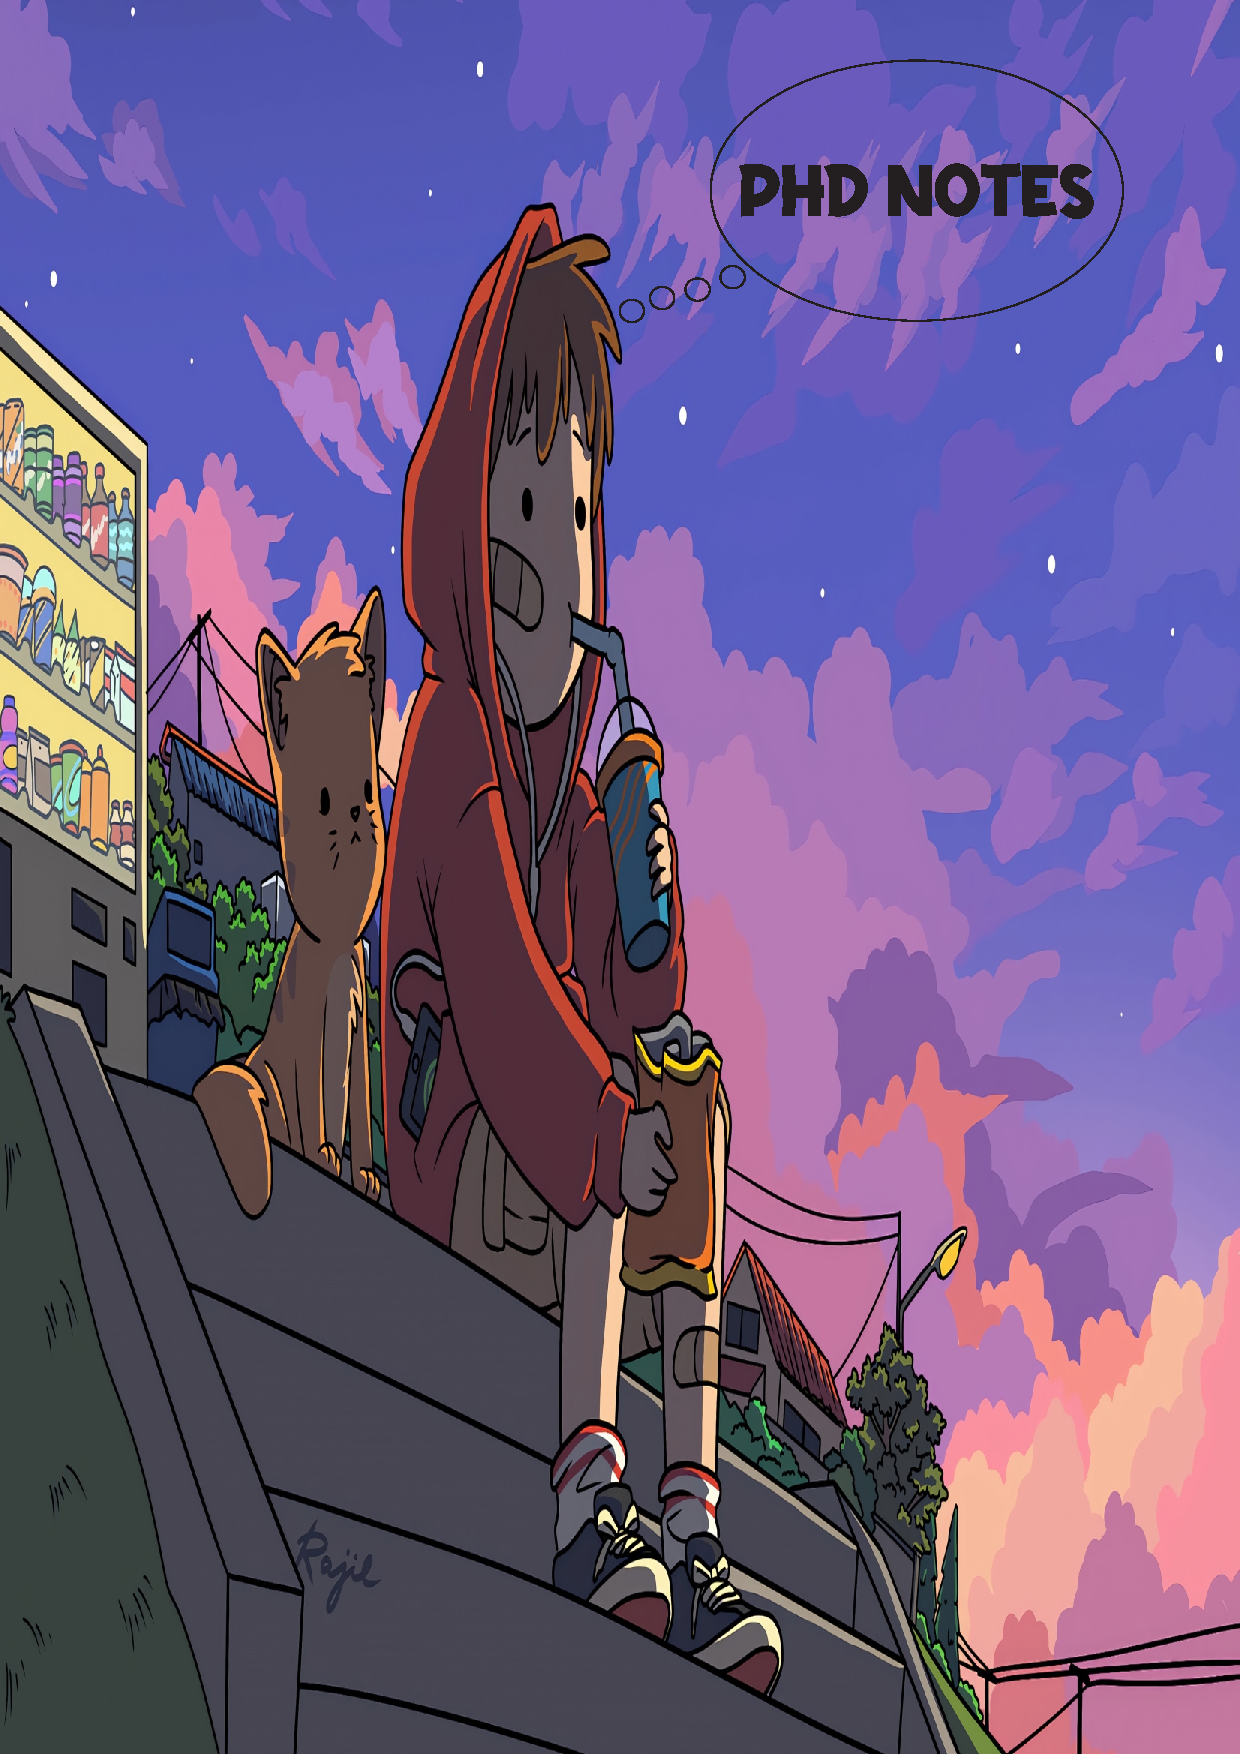
\includepdf[pages={1}]{PhD_Notes_Cover}

\tableofcontents*
\mainmatter


% Include paper chapters (examples)
\chapter[Optimization of Device Geometry in Single-Plate DMF\\{\normalfont Abdelgawad et al. (2009)}]%
{Optimization of Device Geometry in Single-Plate Digital Microfluidics\\[1ex]{\normalfont Abdelgawad et al. (2009)}}

\section{Paper Overview}
\includefig[h!]{0.8}{Abdelgawad_2019_Overview }{Paper overview}
\includefig[h!]{0.8}{Abdelgawad_2019_GeometryComparison}{6 grounding geometries comparison}  % Folder with a tex file for Jane Doe et al 2023
%\documentclass{Notes}

% Metadata
\title{PhD Research Notes}
\author{Farhan Aizuddin}
\date{\today}

\begin{document}

% Roman numbered frontmatter
\frontmatter
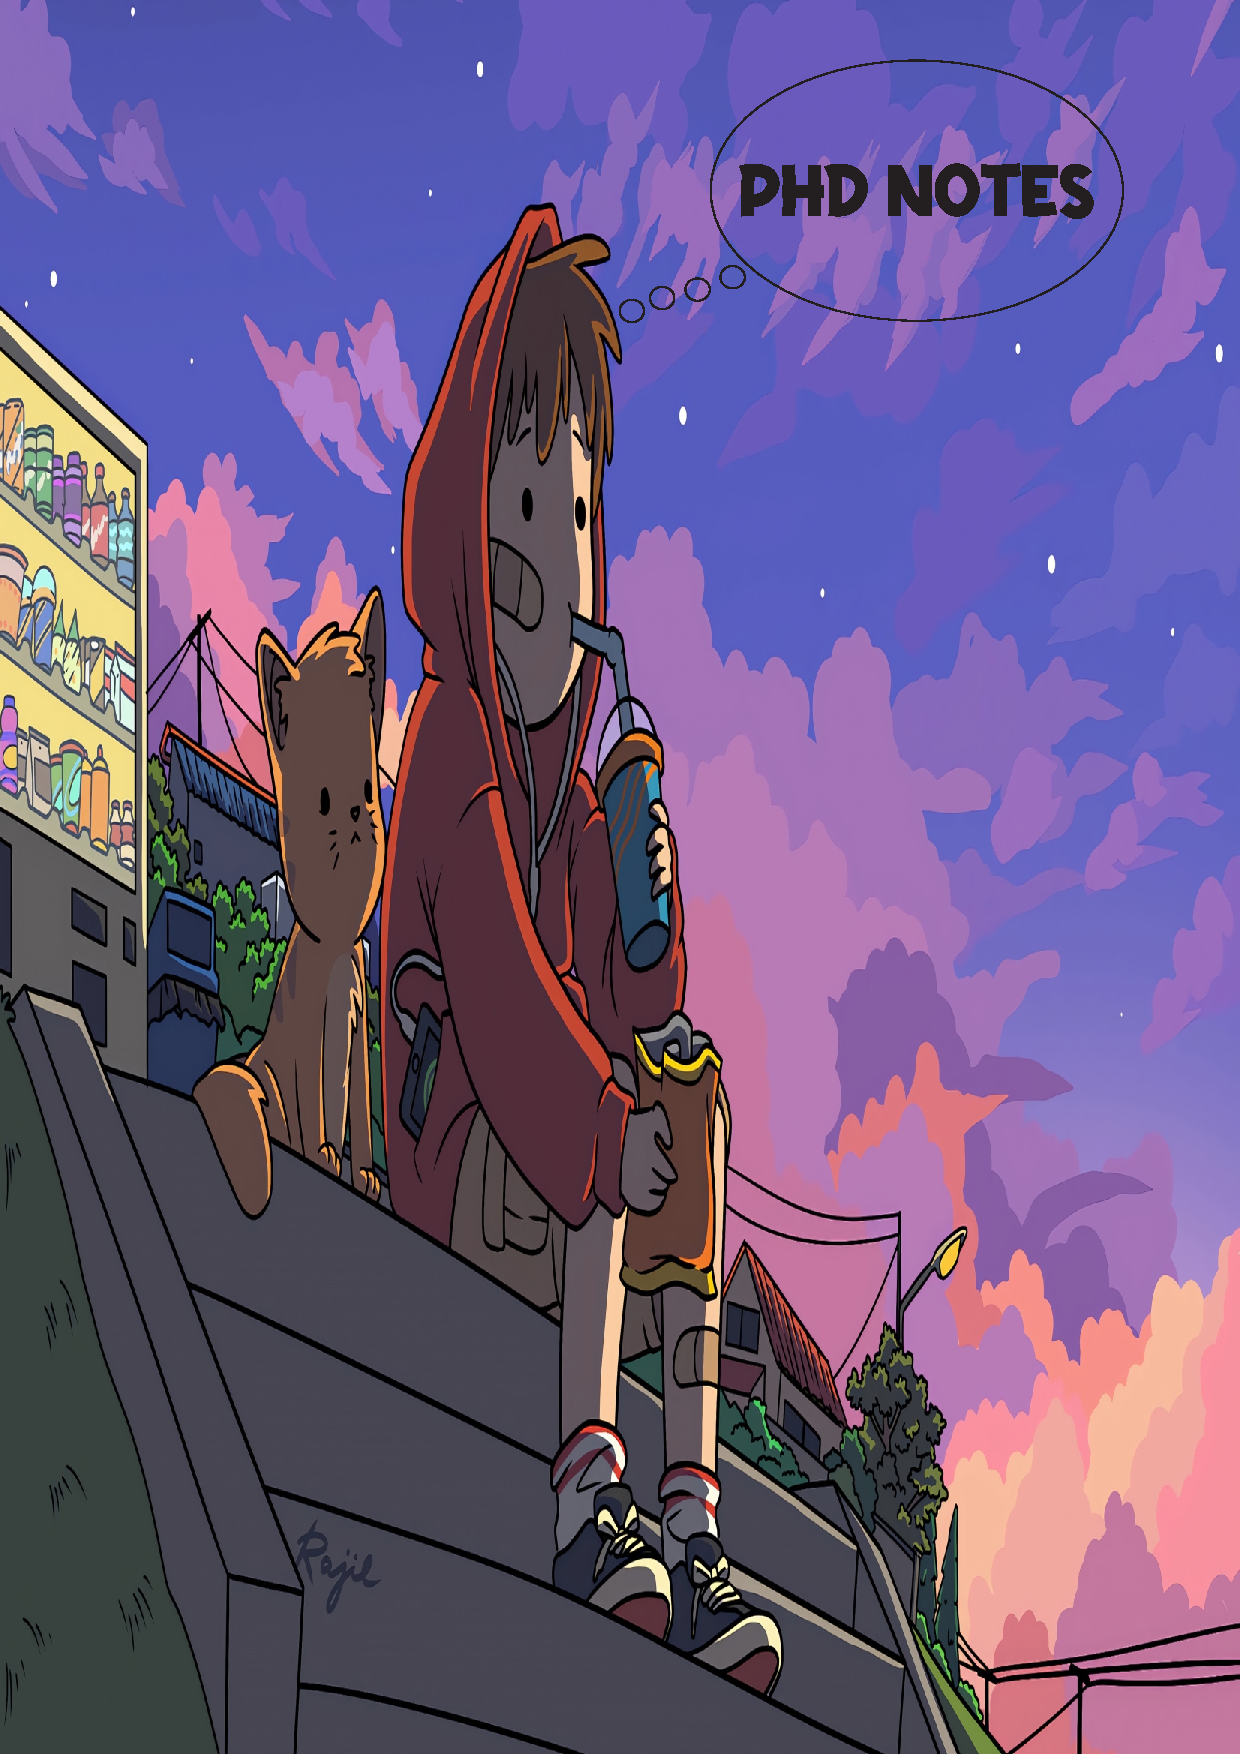
\includepdf[pages={1}]{PhD_Notes_Cover}
\tableofcontents*

% Arabic numbered content
\mainmatter

% Include chapters
\chapter{Introduction}
\section{General Overview}
Salmonella contamination poses a persistent threat to public health, leading to a significant
number of foodborne illnesses worldwide. The conventional methods employed for Salmonella detection often suffer from inherent limitations, hindering the timely and accurate identification of this pathogen. Current techniques, such as culture-based methods and
polymerase chain reaction (PCR), are resource-intensive, time-consuming, and may lack
the sensitivity required for early detection.Additionally, these methods often demand specialized
laboratory equipment and skilled personnel, limiting their applicability in diverse settings, especially in resource-limited environments or during urgent situations.\\

The need for a rapid, cost-effective, and user-friendly Salmonella bacteria detection system is evident, given the severe health consequences associated with delayed identification. Conventional approaches may result in prolonged response times, contributing to the spread of infections and complicating public health interventions. Furthermore, the increasing global interconnectedness of food supply chains necessitates the development of technologies that
can be easily deployed in various settings, including laboratories, agricultural facilities, and field environments.\\

Addressing these challenges requires a paradigm shift towards innovative detection methodologies
that not only enhance sensitivity and specificity but also improve accessibility and affordability. The development of a scalable and portable Digital Microfluidics Platform (DMF) integrated with electrochemical (EC) sensors could provide an insight of which Salmonella bacteria species causes an outbreak.\\

This project aims to contribute to the advancement of public health initiatives and ensure the timely identification of Salmonella, thereby mitigating the impact of foodborne outbreaks
on a global scale.

\section{Problem Statement}
\section{Research Objectives}
\section{Notes Layout}
\section{Problem Statement}
The persistence of salmonella contamination poses a threat to public health, leading to a significant number of foodborne illnesses worldwide. Identifying which salmonella species contributed to an outbreak are often impeded by the inherent limitations of the conventional methods employed for detecting this pathogen such as time-consuming and labor-intensive procedures \cite{silvaRecentDevelopmentsLateral2023}.\\

These techniques also require specialized laboratory equipments, trained staff and large volumes of samples, which limits their usefulness in a variety of contexts, particularly those with low resources or in times of emergency \cite{shenBiosensorsRapidDetection2021,wangOverviewRapidDetection2021}.\\

To address these issues, microfluidic techniques have been employed to reduce the volume of samples and reagents needed for bacteria sample preparation, fast reaction and automatic operation \cite{qiMicrofluidicBiosensorRapid2021,nguyenCompleteProtocolRapid2019} prior for detection procedures via electrochemical (EC) or optical sensors. \\

Microfluidics techniques however involves in designing complex geometries, inclusion of micropumps and microvalves to prepare the samples and produce the necessary results which can be time-consuming \cite{suMicrofluidicsBasedBiochipsTechnology2006}. Therefore, it's necessary to find a different approach when creating a platform that can prepare samples and identify \emph{Salmonella} species without relying on  extra hardware or intricate geometries.\\

DMF is a liquid handling technology which manipulates fluids into discrete droplets on a surface of an array of electrodes through non-contact forces such as electrical, magnetic or thermal \cite{nguyenCompleteProtocolRapid2019,qiMicrofluidicBiosensorRapid2021}.\\

Compared to the microfluidics approach, this method would enable sample volumes to be lowered to nanoliters. Additionally, because the generated sample droplets can be precisely manipulated, samples in droplet form can be further divided into smaller droplets for parallel detection.\newpage 

For bacteria samples identification, optical sensors are often used as compared to EC sensors when combined with DMF-based platform due to the EC sensor lifetime contributed by the rapid dissolution of reference electrode (RE) made up of silver chloride (\ce{AgCl}) \cite{farzbodIntegrationReconfigurablePotentiometric2018}.\\

These systems are, however, expensive and not portable for conducting sample preparation and identification for on-site detection \cite{andersonThinfilmtransistorDigitalMicrofluidics2021}. Hence, this study would investigate and develop a DMF-based platform to be integrated with an array of improved EC sensors to perform \emph{Salmonella} bacteria species detection.\\

Previous works are concentrated on detecting a specific pathogen from a droplet \cite{andersonThinfilmtransistorDigitalMicrofluidics2021,foudehRapidMultiplexDetection2015,luSensitiveAutomatedDetection2023 ,sistaDigitalMicrofluidicPlatform2011} whereby a singular peak detected during the identification process or changes in colour signifies the pathogen existence in the sample. There are ,however ,  less reports on detecting multiple species of a targeted pathogen such as \emph{Salmonella} bacteria.\\

To address this, a probability method such as Fuzzy Logic can be introduced to help in detecting the probability of \emph{Salmonella} bacteria species extisted within the prepared sample. The capability of Fuzzy Logic in determining the pathogen species should be investigated in terms of the sample concentration and voltage resulted from the EC sensor read-out.

\input{Chapters/C1/Objectives/Objective.tex}
\input{Chapters/C1/Scopes/Scope.tex}
\chapter{Literature Review}
\section{General Overview}
Salmonella bacteria are the pathogens that are capable to cause health related problems such as gastroentritis and enteric fever, in which an infection normally be caused by contaminated water and food \cite{bellRecentEmergingInnovations2016,pashazadehNanomaterialsUseSensing2017, pacholewiczEnvironmentalSamplingMethods2023,wangRecentAdvances3D2021}.\\

Current Salmonella detection methods that are available are listed in Figure \ref{CurrSalmDetecMetho} \cite{awangAdvancementSalmonellaDetection2021}. Most of these methods required expensive equipments, well-trained personal and no \textit{in-situ} testing \cite{shenBiosensorsRapidDetection2021,wangOverviewRapidDetection2021}. Furthermore, the time needed to detect the pathogen ranged between several hours to 4 hours  \cite{awangAdvancementSalmonellaDetection2021}.
\begin{figure}[h!]
    \centering
    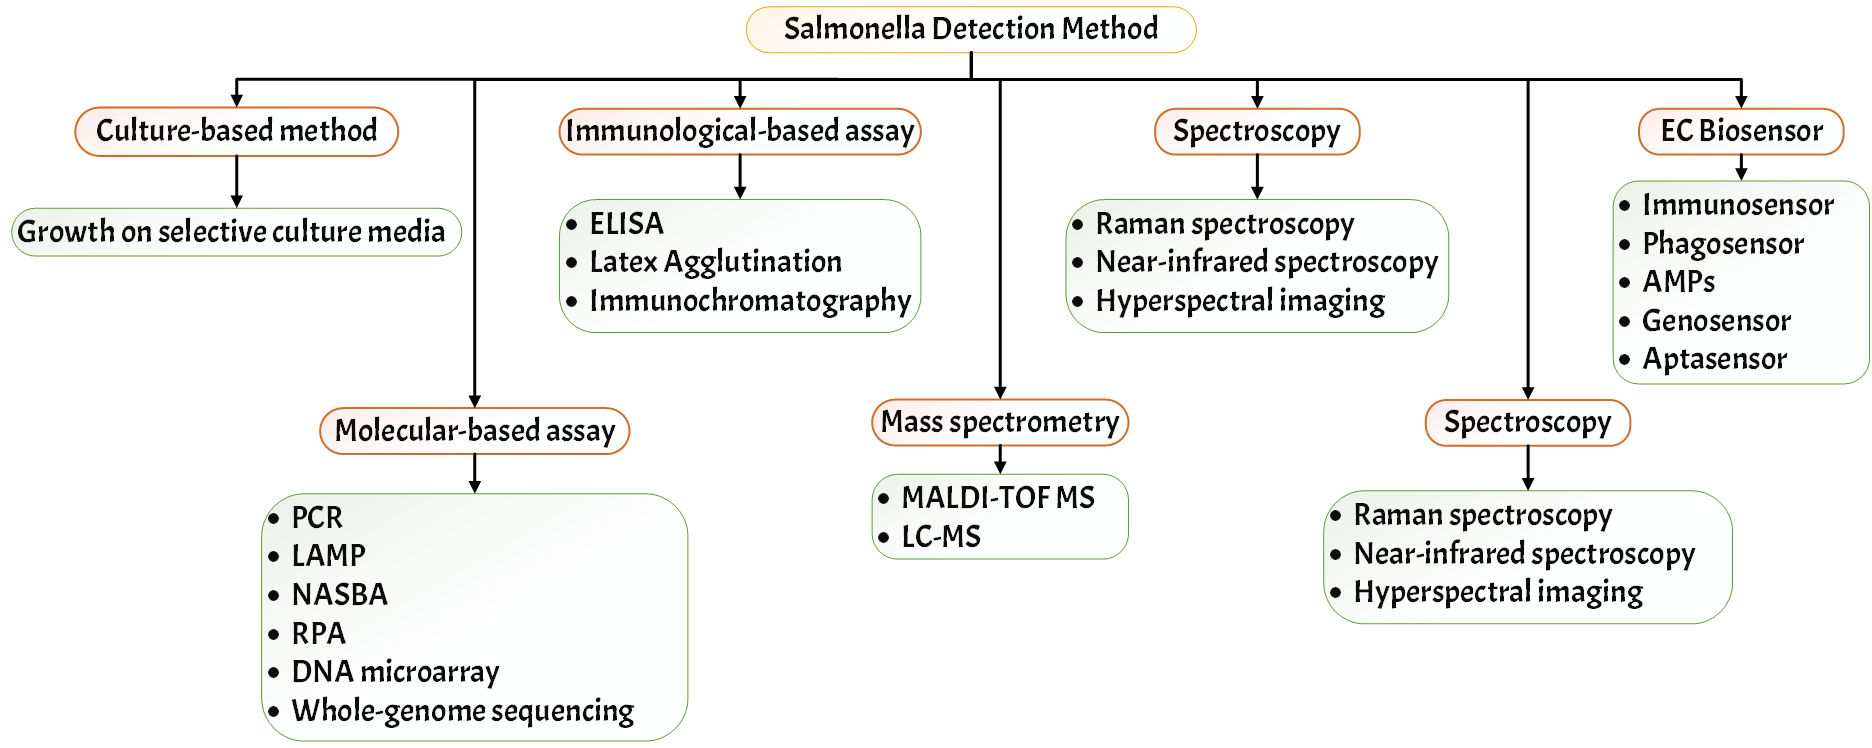
\includegraphics[width=\linewidth]{Figures/Awang_2021_Salmonella_Detection.png}
    \caption{Current available methods for Salmonella detection \\ (adapted from \cite{awangAdvancementSalmonellaDetection2021})}
    \label{CurrSalmDetecMetho}
\end{figure}

Due to these limitations, developments of rapid and sensitive detection methods of this particular pathogen has been researched to prevent another outbreak from occuring. The main concern is the modularity and compatibility with other techniques to have the sample to be tested on site and provide prelimninary finding before the sample is sent to the laboratory for more detail analysis.\newpage

One of the rapid detection methods in the biomedical space is DMF whereby droplets were generated from liquids in microliter (μL) and manipulated on an array of electrodes to perform protocols before the droplets are actuated to the sensing block for detection procedures.\\

This would allow parallel process to be conducted on the same electrodes, which helps in reducing waste and provide economical handling of the samples for on-site testing purposes \cite{agarwalDigitalMicrofluidicsTechniques2012}.\\

The organization of this literature review notes are structured as below:
\begin{enumerate}
    \item Section 2.1 provides general overview on salmonella bacteria
    \item Section 2.2 provides the available methods (conventional/alternative) used for salmonella detection and the advantages/disadvantages of the said methods.
    \item Section 2.3 provides DMF background, timeline of DMF research, and key operations of DMF
    \item Section 2.4 provides available DMF fabrication, actuation and validation methods
    \item Section 2.5 provides the summary of literature review
\end{enumerate}
\section{Salmonella Method of Detection}
Current Salmonella detection methods that are available are listed in Figure \ref{CurrSalmDetecMetho} \cite{awangAdvancementSalmonellaDetection2021}. Most of these methods required expensive equipments, well-trained personal and no \textit{in-situ} testing \cite{shenBiosensorsRapidDetection2021,wangOverviewRapidDetection2021}. Furthermore, the time needed to detect the pathogen ranged between several hours to 4 hours  \cite{awangAdvancementSalmonellaDetection2021}.\\
\begin{figure}[h!]
    \centering
    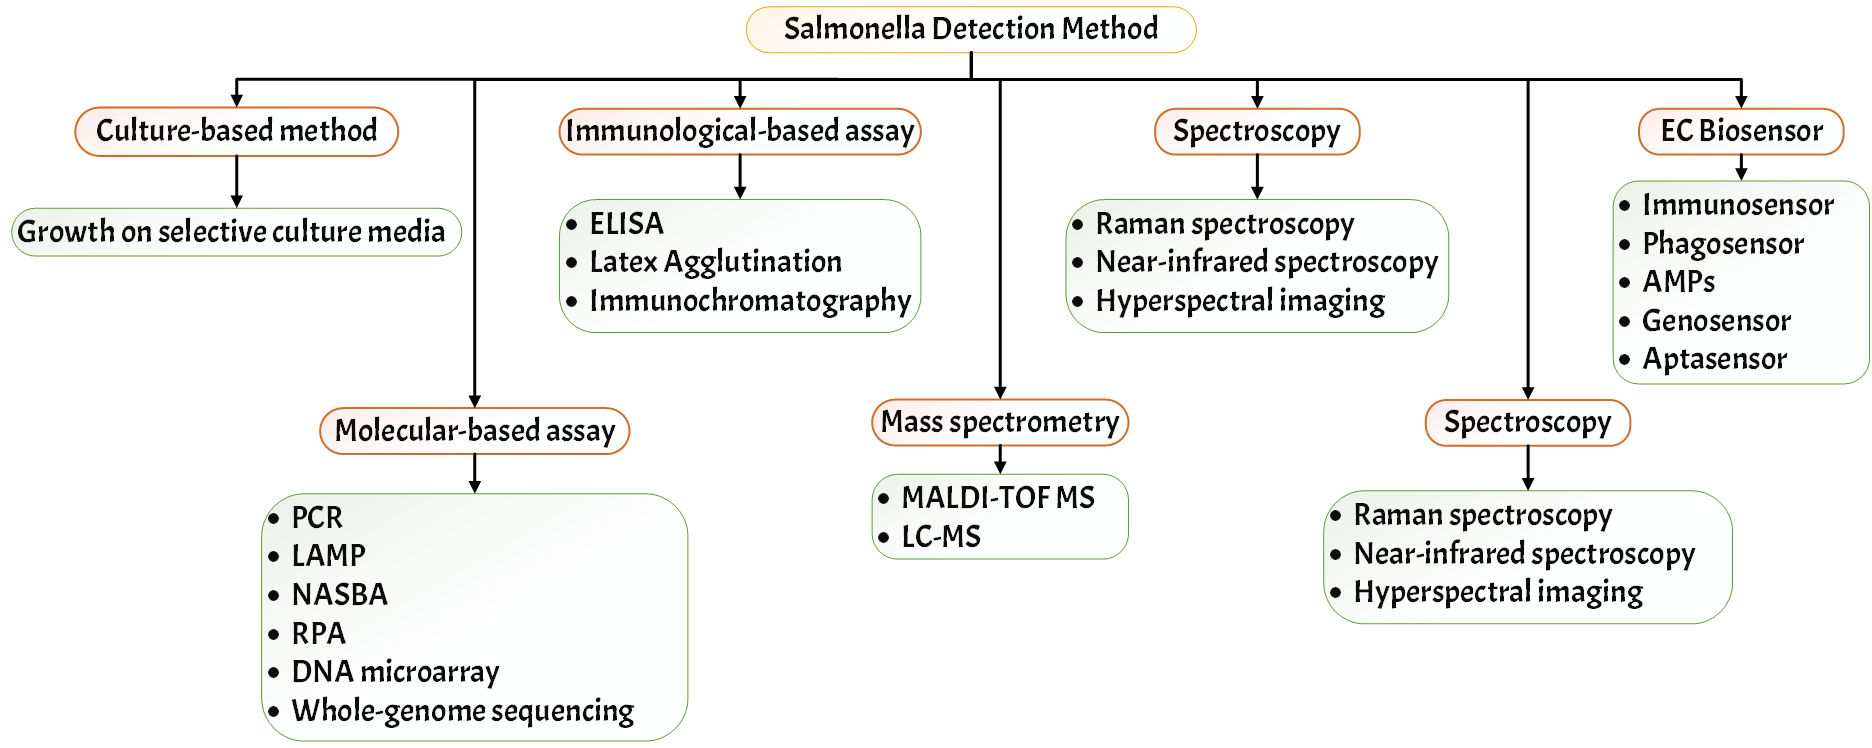
\includegraphics[width=\linewidth]{Figures/Awang_2021_Salmonella_Detection.png}
    \caption{Current available methods for Salmonella detection \\ (adapted from \cite{awangAdvancementSalmonellaDetection2021})}
    \label{CurrSalmDetecMetho}
\end{figure}

Due to these limitations, developments of rapid and sensitive detection methods of this particular pathogen has been researched to prevent another outbreak from occuring. The main concern is the modularity and compatibility with other techniques to have the sample to be tested on site and provide prelimninary finding before the sample is sent to the laboratory for more detail analysis.\newpage

One of the rapid detection methods in the biomedical space is DMF whereby droplets were generated from liquids in microliter (μL) and manipulated on an array of electrodes to perform protocols before the droplets are actuated to the sensing block for detection procedures.\\

This would allow parallel process to be conducted on the same electrodes, which helps in reducing waste and provide economical handling of the samples for on-site testing purposes \cite{agarwalDigitalMicrofluidicsTechniques2012}.\\
\section{Digital Microfluidics (DMF)}
Digital microfluidics (DMF) represents a significant departure from traditional microfluidic techniques. Instead of relying on continuous flow through intricate channel geometries and external micropumps, DMF controls liquid movement by manipulating individual droplets on a planar surface using localized electric fields applied on an array of electrodes \cite{abdelgawadDigitalRevolutionNew2009,fairChemicalBiologicalApplications2007}.\\

Due to smaller form factor, DMF allows smaller liquid volume for laboratory processes to be in microliter (\textmugreek L) and picoliter (pL), thus reducing reagents and samples wastage \cite{bhattacharjeeDropletPositionControl2010,royNewSamplePreparation2015}.\\

Another advantage of DMF have over microfluidics are reduced sample cross-contamination and dispersion. This is due to the droplet served as a self-contained microreactor, there is negligible cross-mixing between different samples or reagents \cite{luoMachineVisionbasedDriving2021,wuResearchProgressElectrode2023}.\newpage

\subsection{Architecture}
DMF are categorically divided into two configurations, which are open and closed as illustrated in Figure \ref{DMFConfig}.\\
\begin{figure}[h!]
    \centering
    \begin{subfigure}{0.45\textwidth}
        \centering
        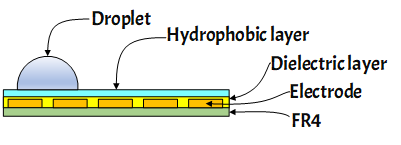
\includegraphics[width=\textwidth]{Open_TypeDMF.png}
        \caption{Open type DMF}
        \label{OpenTypeDMF}
    \end{subfigure}
    \begin{subfigure}{0.45\textwidth}
        \centering
        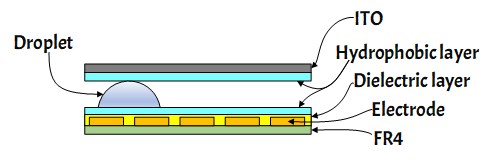
\includegraphics[width=\textwidth]{Closed_TypeDMF.png}
        \caption{Closed type DMF}
        \label{ClosedTypeDMF}
    \end{subfigure}
    \caption{Types of DMF configurations using FR4 as the substrate}
    \label{DMFConfig}
\end{figure}

Open-configuration DMF constitutes of a substrate where an array of electrodes (actuation and grounding connections included), a layer of dielectric layer and a layer of hydrophobic layer are deposited on top of it. Grounding methods for open-type DMF exhibit greater variability and may include a conductive probe inserted into the droplet, exposed ground traces interspersed between actuation electrodes, or subsurface grounding electrodes embedded below the dielectric layer \cite{yafiaDigitalMicrofluidicSystems2018}. The absence of an upper confining substrate results in the droplet interface being exposed to ambient conditions or, in certain implementations, immersed in a continuous oil phase to suppress evaporation and enhance droplet stability \cite{vafaieNumericalSimulationEWOD2019,yafiaHighPrecisionControl2013,yafiaLowCostGrapheneBasedDigital2020}. \\

The dielectric layer electrically isolates the actuating electrode array, thereby suppressing leakage currents and inhibiting electrolysis. A hydrophobic coating is deposited atop the dielectric to lower the surface energy and minimize droplet pinning \cite{abdelgawadDigitalRevolutionNew2009,agarwalDigitalMicrofluidicsTechniques2012,barmanElectrowettingondielectricEWODCurrent2020,jebrailLetsGetDigital2010}. Droplet actuation and transport are achieved through modulation of the interfacial forces under an applied electric field.\\

In the closed configuration, droplets are confined within the gap between two parallel substrates \cite{abdelgawadOptimizationDeviceGeometry2009,al-lababidiMinimumMovableDroplet2023}. The lower substrate incorporates a patterned electrode array for actuation, while the upper substrate—typically a continuous ground plane—is often fabricated from a transparent conductive material such as Indium Tin Oxide (ITO) to enable optical observation \cite{barmanElectrowettingondielectricEWODCurrent2020,sukthangRapidFabricationCloseTyped2020}. \\

Both the actuation electrodes on the bottom substrate and, in many cases, the ground electrode on the top substrate are coated with a dielectric layer to isolate the droplet and preventing electrolysis and dielectric breakdown. A hydrophobic coating is further applied to both surfaces to reduce contact angle hysteresis and enhance droplet mobility \cite{agarwalDigitalMicrofluidicsTechniques2012,jebrailDigitalMicrofluidicsVersatile2012,meimandiDevelopmentElectrowettingDigital2019}.\newpage

\subsection{Droplet Manipulation Techniques}

\subsection{Core Operations}
Generally, key droplet operations that can be executed by DMF are shown in Figure \ref{DMFOps} \cite{bhattacharjeeMultipleDilutionSample2012,bhattacharjeeEfficientGenerationDilution2019,bhattacharyaAlgorithmicChallengesDigital2014}.
\begin{figure}[h!]
    \smartdiagramset{bubble node font=\sffamily\large,
    bubble center node font=\sffamily\Huge}
    \centering
    \smartdiagram[bubble diagram]{
        DMF\\Operations,
        Transport,
        Merging,
        Splitting,
        Dispensing,
        Mixing,
        Storage,
        Sensing
        }
    \caption{DMF key operations}
    \label{DMFOps}
\end{figure}

\input{Chapters/C2/Summary/C2_Summary.tex}
\input{Chapters/C3/General_Flow/ResearchFlow.tex}
\input{Chapters/C3/DMF_DesignFabrication/Design_Fabrication.tex}
\input{Chapters/C3/Droplet_Actuation/Driver_Design.tex}
\input{Chapters/C3/Movement/DMF_Movement.tex}
\input{Chapters/C3/DMF_Integration/DMF_EC_Integration.tex}
\input{Chapters/C3/Data_Collection/Data.tex}
\input{Chapters/C3/Summary/C3_Summary.tex}

% Bibliography
\backmatter
\bibliographystyle{IEEEtran}
\bibliography{Papers}


\end{document} % Another paper

%\printbibliography

\end{document}
